% !TeX root = ../UrrutiaAnguiano_CandidaturaDefensa.tex
% !TeX spellcheck = es_MX 

\section{Antecedentes y objetivos del proyecto}

%----------------------------------------------------------------------------------
%----------------------------------------------------------------------------------
\begin{frame}[t]{Antecedentes}
	{\textoverline{Metasuperficies para biosensado}}
	
	\vskip1em%
	\hskip3em%
	\begin{beamercolorbox}[wd=1.3\squeezethree]{}
		\emphr{Metasupercie plasmónica:} Arreglo bidimensional de nanoestructuras metálicas
		soportadas por un sustrato.\footnotemark[1]\\[1em]
		
		Sintonización de propiedades ópticas:
		\begin{itemize}  
			\item Geometría
			\item Material
			\item Distribución espacial
		\end{itemize}
		\vskip1em
		Esquemas de medición:
		\begin{itemize}
				\item Reflexión\footnotemark[2]
				\item Elipsometría\footnotemark[3]$^,$\footnotemark[4]
		\end{itemize}
	\end{beamercolorbox}%
	
	\begin{textblock*}{40mm}(80mm,50mm)\scriptsize
		\rule{20mm}{.5pt}\\
		\footnotemark\fullcite{gonzalez-alcalde_large_2020}
	\end{textblock*}
	
	
	% Nanorods kabashin_plasmonic_2009 -------------------------------
	\begin{textblock*}{1mm}(140mm,10mm)
		\begin{tikzpicture}[font=\scriptsize]
			\node (img) {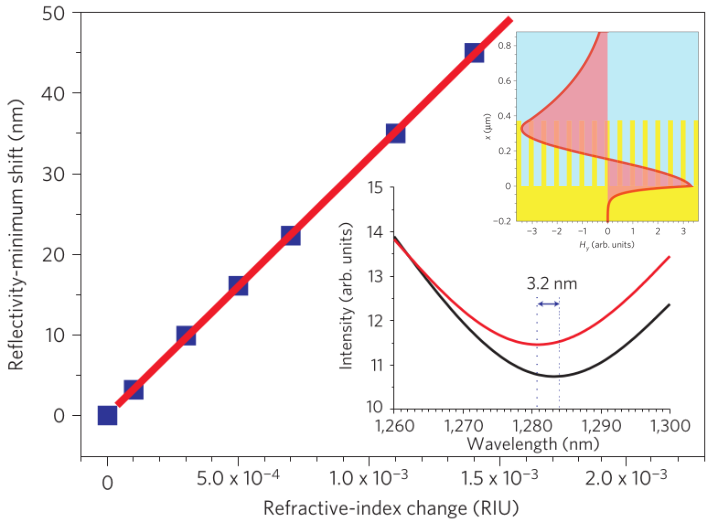
\includegraphics[width = 85mm]{img/0-Intro/kabashin-1.png}};
			\path (img.200) node [anchor = east, xshift= 0mm] {\begin{minipage}{40mm}
					\begin{flushright}
						\rule{20mm}{.5pt}\\
						\footnotemark[2]\fullcite{kabashin_plasmonic_2009} \\[1em]
						Crecimiento electroquímico
						Au/Al$_2$O$_3$\\[1em]
						$L = 380$~nm\\
						$a = 12.5$~nm\\
						$\Lambda = 60$~nm
					\end{flushright}
			\end{minipage}};	
\uncover<2->{
			\path (img.135) node[anchor = north west, xshift = -2mm]{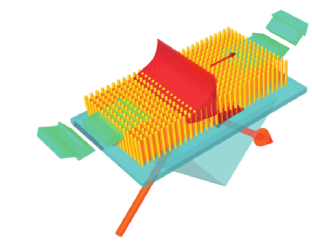
\includegraphics[width = 35mm]{img/0-Intro/kabashin-2.png}};
}
		\end{tikzpicture}
	\end{textblock*}
	
	% COVID qiu_dual_2020 -----------------------------------------
	\begin{textblock*}{1mm}(40mm,90mm)
		\begin{tikzpicture}[font=\scriptsize]
			\node (img) {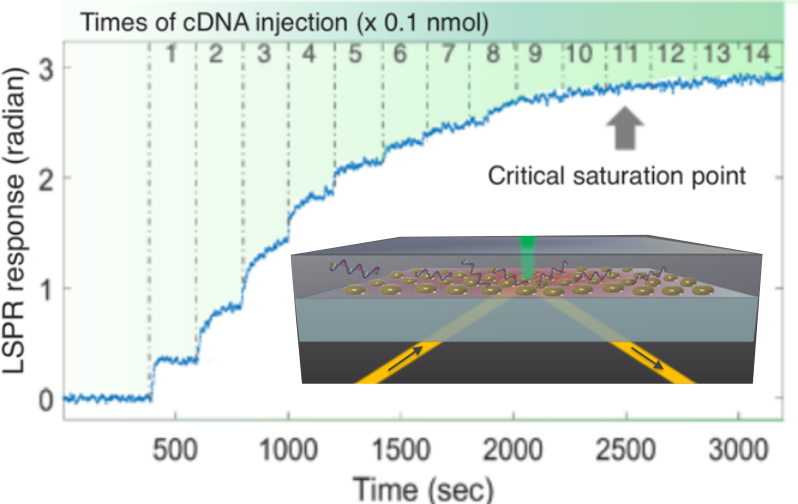
\includegraphics[width = 85mm]{img/0-Intro/qiu-1.png}};
			\path (img.0) node [anchor = north west, xshift=-2.5mm] {\begin{minipage}{30mm}
					\begin{flushleft}
						\rule{20mm}{.5pt}\\
						\footnotemark[3]\fullcite{qiu_dual_2020} \\[1em]
						Dewetting\\[1em]
						$d = 5$~nm\\
						(Grosor película)
					\end{flushleft}
			\end{minipage}};	
		\end{tikzpicture}
	\end{textblock*}

	% Sensor qiu_dual_2015 -----------------------------------------
	\begin{textblock*}{1mm}(140mm,80mm)
\uncover<2->{		\begin{tikzpicture}[font=\scriptsize]
			\node (img) {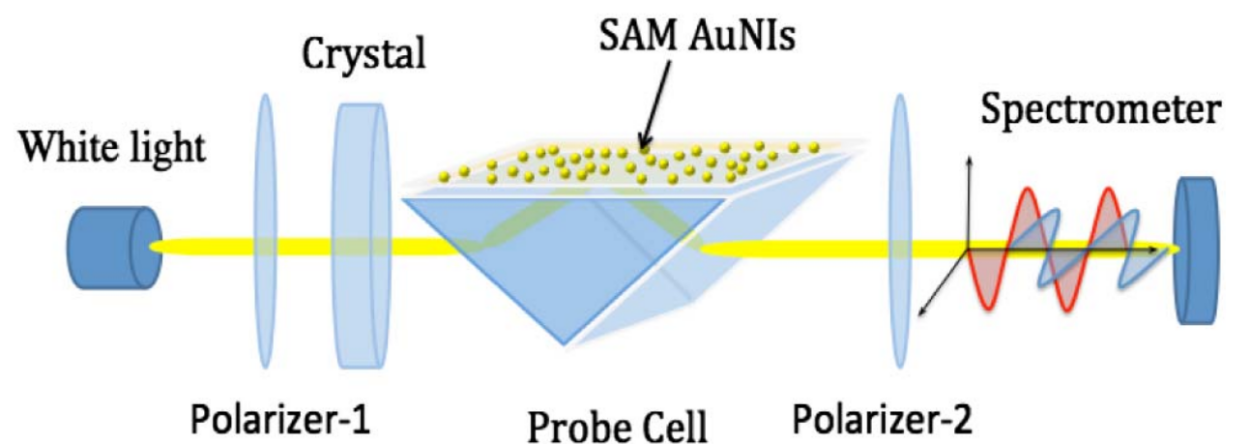
\includegraphics[width = 85mm]{img/0-Intro/qiu-2.png}};
			\path (img.350) node [anchor = north, yshift= -6mm] {\begin{minipage}{60mm}
					\begin{flushleft}
						\rule{20mm}{.5pt}\\
						\footnotemark[4]\fullcite{qiu_differential_2015}
					\end{flushleft}
			\end{minipage}};	
		\end{tikzpicture}
}
	\end{textblock*}


\end{frame}

%----------------------------------------------------------------------------------
\begin{frame}[c]{\underline{Metasuperficies en condiciones realistas}}
	{Polidispersidad y efectos de sustrato}
	\begin{center}
	\begin{tikzpicture}[node distance=20mm and 50mm,font=\normalsize]

	% Conceptos -----------------------------------------
		\path (0,0) node[concept](poli) {Polidispersidad de tamaños};
		\node[concept, right=of poli] (sus) {Presencia del sustrato};
		\node[concept, right=of sus] (emb) {Incrustamiento};

	% Wang Polidispersidad -----------------------------------------
		\node[below=of poli] (wang) {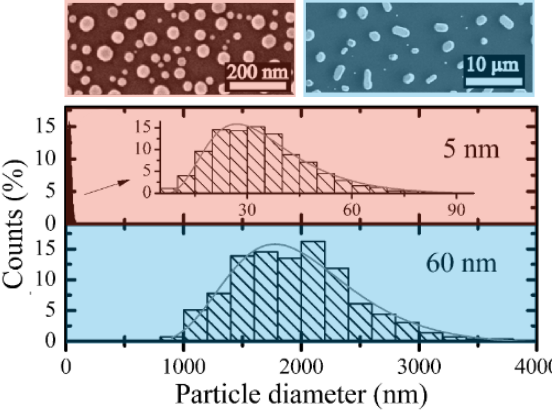
\includegraphics[width = 80mm]{img/0-Intro/wang.png}};
		\draw[hidden] (poli.south) --
			node[above,text=sdgrayFC,font=\itshape,anchor=west] {Enfoque analítico}
			  (wang.90 -| poli.south);%
		\path (wang.300) node [anchor = north, yshift= 0mm,font=\scriptsize] {\begin{minipage}{40mm}
				\begin{flushright}
					\rule{20mm}{.5pt}\\
					\fullcite{wang_formation_2011}
				\end{flushright}
			\end{minipage}};

	% Bohra Sustrato -----------------------------------------				
		\node[below=of sus, xshift=-7.5mm] (borah) {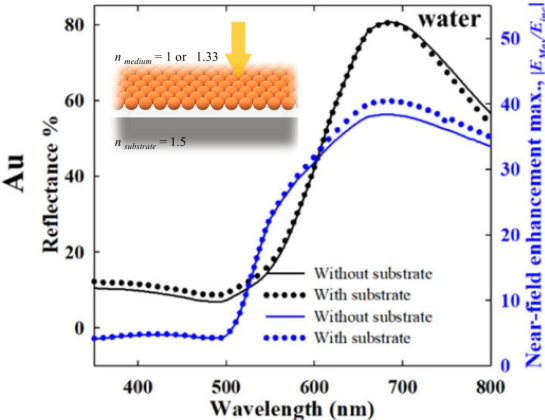
\includegraphics[width = 80mm]{img/0-Intro/borah.png}};
		\draw[hidden] (sus.south) --
				node[above,text=sdgrayFC,font=\itshape,anchor=west] {
					\begin{minipage}{40mm}
						Enfoque analítico\\
						Cálculo numérico
					\end{minipage}}
				(borah.90 -| sus.south);%
		\path (borah.300) node [anchor = north, yshift= 0mm,font=\scriptsize] {\begin{minipage}{40mm}
				\begin{flushright}
					\rule{20mm}{.5pt}\\
					\fullcite{borah_plasmon_2022}
				\end{flushright}
		\end{minipage}};

	% Moirangthem Incrustación -----------------------------------------	
		\node[below=of emb] (mori) {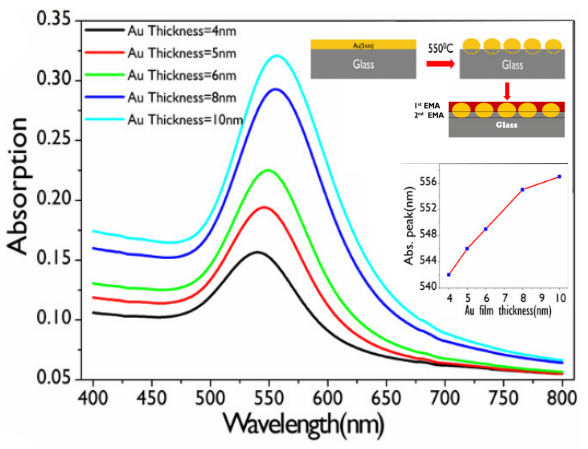
\includegraphics[width = 80mm]{img/0-Intro/moirangthem.png}};
		\draw[hidden] (emb.south) --
			node[above,text=sdgrayFC,font=\itshape,anchor=west] {
				\begin{minipage}{40mm}
					Enfoque analítico\\
					Cálculo numérico
			\end{minipage}}
			(mori.90 -| emb.south);%		
		\path (mori.300) node [anchor = north, yshift= 0mm,font=\scriptsize] {\begin{minipage}{40mm}
				\begin{flushright}
					\rule{20mm}{.5pt}\\
					\fullcite{moirangthem_enhanced_2012}
				\end{flushright}
		\end{minipage}};
	\end{tikzpicture}
\end{center}
\end{frame}

%----------------------------------------------------------------------------------
\begin{frame}[t]{\underline{Respuesta óptica de metasuperficies}}
	{Enfoques analíticos}
\begin{center}
\begin{columns}
	\column{.95\squeezetwo}
	\centering
	% Medio efectivo -----------------------------------------	
	\begin{block}{\centering  Teorías de medio efectivo\footnotemark[1]}
		\vskip1em
		\begin{itemize}
			\item Remplazo de incrustaciones en un   material por un \emphr{medio homogéneo}
			\item \emphr{Ejemplos:} Maxwell Garnett y Bruggeman
			\item Usualmente para sistemas coloidales
			\item \emphr{Correcciones }fenomenológicas para uso en metasuperficies\footnotemark[2]
		\end{itemize}	
	\centering\vskip1em
	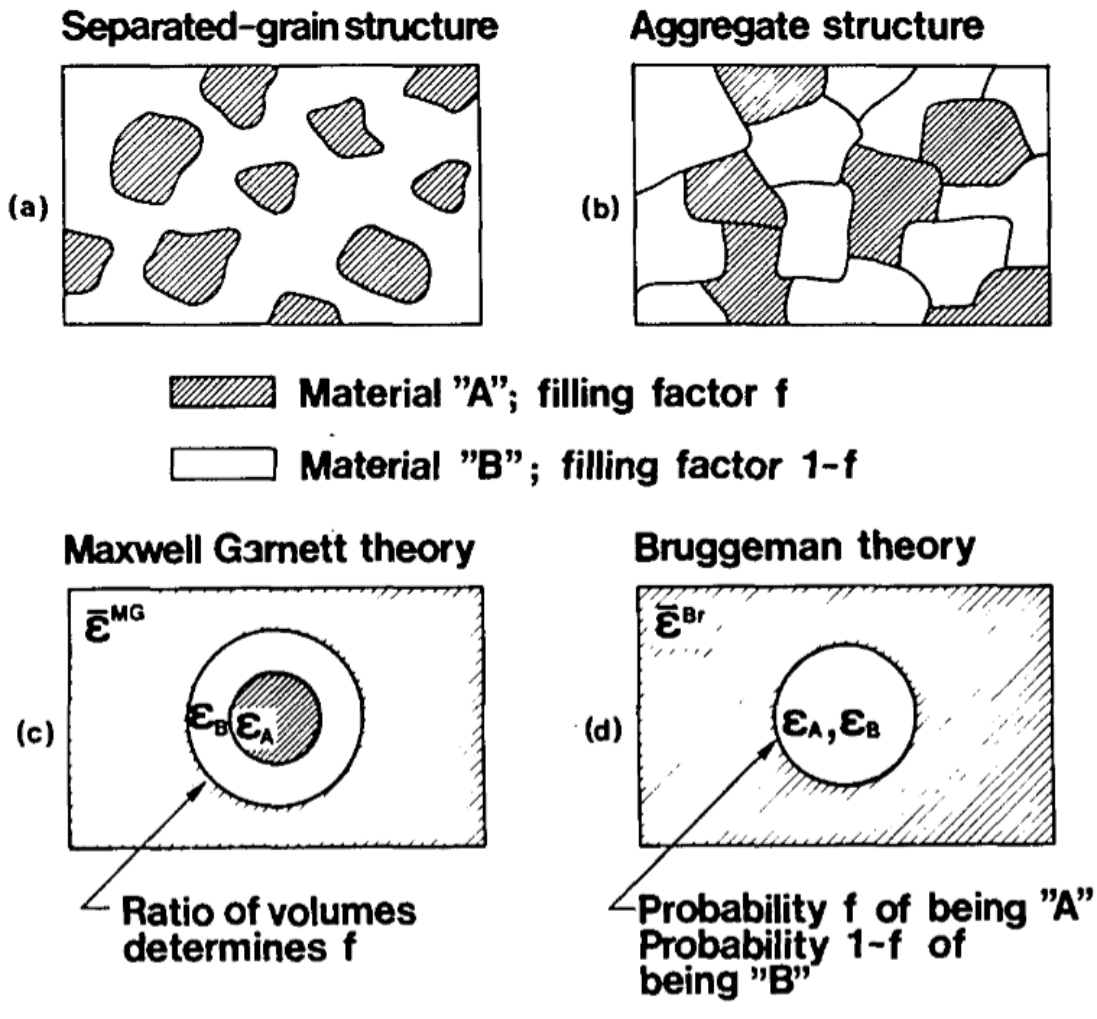
\includegraphics[width = 80mm]{img/0-Intro/niklasson.png}
	\vspace{-1em}\begin{flushright}\scriptsize
		\rule{20mm}{.5pt}\\
		\footnotemark[1]\fullcite{niklasson_effective_1981}\\
		\footnotemark[2]\fullcite{kabashin_plasmonic_2009}
	\end{flushright}
	\end{block}

	% Esparcimiento Múltiple -----------------------------------------	
	\column{.8\squeezetwo}
	\centering
	\begin{alertblock}{\centering Teorías de esparcimiento múltiple\footnotemark[3]}
		\vskip1em
		\begin{itemize}
			\item \emphr{Ensamble de partículas} interactuantes
			\item Solución aproximada a las ecuaciones de Maxwell
			\item \emphr{Ejemplos:} Modelo de Esparcimiento Coherente\footnotemark[4] (CSM)\\
					\phantom{\emphr{Ejemplos:}} Teoría de Película Delgada\footnotemark[5] (TFT)
			\item Varios órdenes de aproximación:
				\begin{itemize}
					\item En el orden del esparcimiento múltiple
					\item En el orden multipolar de cada esparcidor
				\end{itemize}
		\end{itemize}	
		\centering\vskip1em
		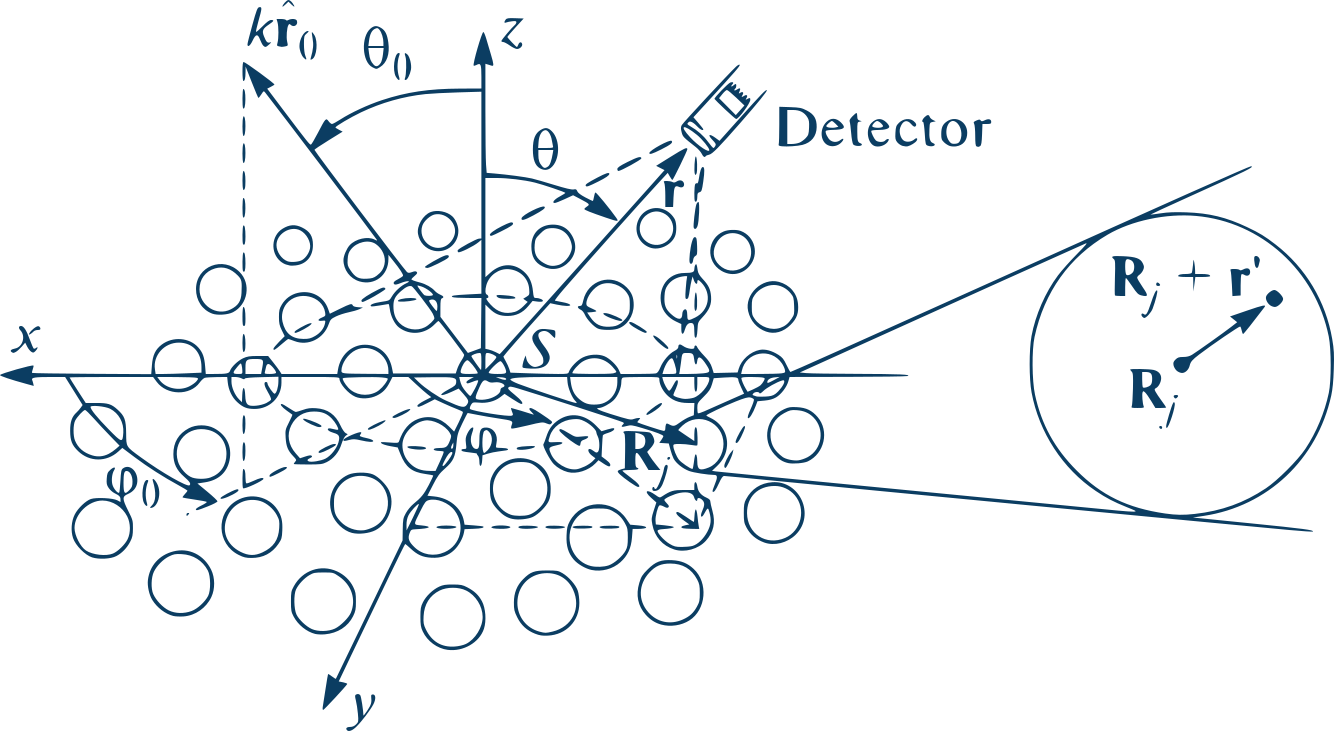
\includegraphics[width = 90mm]{img/0-Intro/loikoB.png}
			\vskip-2em%
			\begin{flushright}\scriptsize
			\rule{20mm}{.5pt}\\
			\footnotemark[3]\fullcite{loiko_scattering_2020}\\
			\footnotemark[4]\fullcite{reyes2018analytical}\\
			\footnotemark[5]\fullcite{bedeaux_optical_2004}
		\end{flushright}
	\end{alertblock}
	\end{columns}
	\end{center}
\end{frame}



\begin{frame}{Objetivos}
	{\textoverline{Colaboración teórico-experimental}}
	\begin{center}
		\begin{tikzpicture}[node distance=20mm and 30mm,font=\normalfont]
			%        \setlength{\leftmargini}{10pt}
			
			% caract
			\node[flowbox] (general) {%
				\fbtitle{Objetivo general}\vphantom{yÖ}
				\nodepart{two}
				\begin{minipage}{.35\textwidth}
					Identificar \textbf{teóricamente} efectos de sustrato y esparcimiento múltiple en \textbf{metasuperficies plasmónicas desordenadas} y contrastar con \textbf{datos experimentales}.
				\end{minipage}
			};
			
			\node[concept, below =of general, align=center,yshift=10mm] (part) {Objetivos particulares};
			\draw[conn] (general.south) -- (part.north);
			
			% imp
			\node[flowbox,below left=of part] (imp) {%
				\fbtitle{Implementación}\vphantom{yÖ}
				\nodepart{two}
				\begin{minipage}{.24\textwidth}
				Métodos analíticos y numéricos
					\begin{itemize}\itemsep0em  \small
						\item CSM\footnotemark[1] y TFT\footnotemark[2]
						\item Descenso de gradiente (Barzilai-Borwein)\footnotemark[3]
						\item COMSOL Multipysics$^\text{TM}$ ver. 6.1
						\item Constraste con mediciones
					\end{itemize}
				\end{minipage}
			};
			
			% efects
			\node[flowbox,below=of part] (efects) {%
				\fbtitle{Cuantificación}\vphantom{yÖ}
				\nodepart{two}
				\begin{minipage}{.24\textwidth}
				\emphr{Caracterización de metasuperficie sintetizada en INAOE}
					\begin{itemize}\itemsep0em  \small
						\item Incrustaminto parcial
						\item Contraste con cálculo numérico
						\item \emphb{Mediciones para estudio de incrustamiento}
					\end{itemize}
				\end{minipage}
			};
			
			% efects
			\node[flowbox,below right=of part] (dis) {%
				\fbtitle{Diseño}\vphantom{yÖ}
				\nodepart{two}
				\begin{minipage}{.24\textwidth}
				Metasuperficie enfocado en biosensado
					\begin{itemize}\itemsep0em  \small
						\item Dos morfologías (CSM y TFT)
						\item Esquema de medición de fase
						\item \emphb{Corrimiento al azul}
					\end{itemize}
				\end{minipage}
			};
			
			\draw[conn] (part.west) -| (imp.north);
			\draw[conn] (part.south) -| (efects.north);
			\draw[conn] (part.east) -| (dis.north);
		\end{tikzpicture}
	\end{center}
	
	\begin{textblock*}{1mm}(200mm,10mm)
		\begin{tikzpicture}[font=\normalfont]
			\node (img) {
\includegraphics[width = 50mm]{img/0-Intro/colab.png}};
			\path (img.270) node [anchor = north] {\begin{minipage}{65mm}
						\emphr{Instituto Nacional de Astrofísica, Óptica y Electrónica (INAOE)}\\
						\emphb{Facultad de Ciencias (FC-UNAM)}
			\end{minipage}};	
		\end{tikzpicture}
	\end{textblock*}
	
	\begin{textblock*}{85mm}(190mm,130mm)
		\begin{flushleft}
		\scriptsize
				\rule{30mm}{.5pt}\\
				\footnotemark[1]\fullcite{reyes2018analytical}\\
				\footnotemark[2]\fullcite{bedeaux_optical_2004}\\
				\footnotemark[3]\fullcite{barzilai_two-point_1988}
		\end{flushleft}
	\end{textblock*}
\end{frame}